% Solutions to the exercises of Chapter 2. Numbers: code/solutions/sol02.py
\documentclass[../solutions_manual.tex]{subfiles}
\begin{document}
\ifSubfilesClassLoaded{\setcounter{chapter}{1}}{}% NN-1 when built standalone
\setcounter{chapter}{1}% NN-1, so this chapter is numbered NN
\chapter{Welfare Theorems as Matrix Properties}\label{sol02}
\sloppy

All numbers below are printed by \texttt{python3 code/solutions/sol02.py}. Throughout, $\Var(\pi_i) = \frac1N\sum_i(\pi_i - \frac1N)^2$ and $\Gamma = 1 - |\lambda_2|$ (Chapter~1, Section~\ref{ch01:sec:conventions}).

%% ---------------------------------------------------------------------
\exercisesolution{2.1}{Doubly stochastic check}

All four matrices are row-stochastic and irreducible. For such $W$, $\boldsymbol\pi = \frac1N\ones$ if and only if every column sums to one (Proposition~\ref{ch01:prop:pi_uniform}), so the test is the column sums.

\solpart{a} Column sums $(1,1,1)$: doubly stochastic. $\boldsymbol\pi = \frac13\ones$, $\Var(\pi_i) = 0$. (Also $\Gamma = 1$: the matrix is $W^{CE}$.)

\solpart{b} Column sums $(0.6+0.1+0.3,\ 0.3+0.6+0.1,\ 0.1+0.3+0.6) = (1, 1, 1)$. The matrix is a circulant, so it is doubly stochastic: $\boldsymbol\pi = \frac13\ones$, $\Var(\pi_i) = 0$. Its other eigenvalues are $0.6 + 0.3\omega + 0.1\omega^2$ with $\omega = e^{\pm 2\pi i/3}$, i.e.\ $0.4 \pm 0.1732i$, of modulus $0.4359$, so $\Gamma = 0.5641$. The matrix is asymmetric and non-anonymous, yet power is equal.

\solpart{c} Column sums $(1.3, 0.7)$: not doubly stochastic. With $W = \begin{pmatrix}1-a & a\\ b & 1-b\end{pmatrix}$, $a = 0.2$, $b = 0.5$, Chapter~3, Proposition~\ref{ch03:prop:block_spectral}(2) gives $\boldsymbol\pi = (b, a)/(a+b) = (5/7, 2/7) = (0.7143, 0.2857)$. Check: $\frac57\cdot0.8 + \frac27\cdot0.5 = \frac{4 + 1}{7} = \frac57$. Then $\Var(\pi_i) = \frac12[(\frac57 - \frac12)^2 + (\frac27 - \frac12)^2] = (\frac{3}{14})^2 = 0.04592$, and $\Neff = 1.6897$. The other eigenvalue is $1 - a - b = 0.3$, so $\Gamma = 0.7$.

\solpart{d} The matrix is symmetric with unit row sums, hence doubly stochastic: $\boldsymbol\pi = \frac13\ones$, $\Var(\pi_i) = 0$. Its eigenvalues are $1$ and $0.1$ (twice), so $\Gamma = 0.9$.

\emph{Lesson.} Matrices (b) and (d) have equal power and different integration ($\Gamma = 0.5641$ and $0.9$); (c) has unequal power and $\Gamma = 0.7$. Power and the gap are separate coordinates. \emph{Common mistake:} concluding from asymmetry, as in (b), that power is unequal.

%% ---------------------------------------------------------------------
\exercisesolution{2.2}{Is there a clawback?}

The setting is Example~\ref{ch02:ex:transfer_vs_structural}: $N = 4$, $\Omega = 20$, $\bar d = 3$, $\Phi = 8$, $\kappa = 0.1$ and $\boldsymbol\pi = (\frac13, \frac13, \frac16, \frac16)$.

\solpart{a} A transfer $\tau$ of disagreement payoff from Agent~2 to Agent~3 gives $\mathbf d' = (3, 3 - \tau, 3 + \tau, 3)$. The total $\sum_j d'_j = 12$ is unchanged, so the surplus is still $\Phi = 8$ and $x'_i = d'_i + 8\pi_i$ (Proposition~\ref{ch01:prop:nash_division}):
\begin{center}
\begin{tabular}{lcccc}
\toprule
$\tau$ & $x'_1$ & $x'_2$ & $x'_3$ & $x'_4$ \\
\midrule
0.5 & 5.6667 & 5.1667 & 4.8333 & 4.3333 \\
1   & 5.6667 & 4.6667 & 5.3333 & 4.3333 \\
2   & 5.6667 & 3.6667 & 6.3333 & 4.3333 \\
3   & 5.6667 & 2.6667 & 7.3333 & 4.3333 \\
\bottomrule
\end{tabular}
\end{center}
Agent~3 receives exactly $\tau$ more than her baseline $4.3333$ in every case, and Agent~2 exactly $\tau$ less: no clawback, as in Proposition~\ref{ch02:thm:transfer_trap}(1). Checks: every row sums to 20, and $\max_i\kappa x'_i \le 0.733 < 1$. The power terms $\pi_i\Phi = (2.667, 2.667, 1.333, 1.333)$ are untouched (part~(2) of the proposition).

\solpart{b} With the gas block's cross-block entry equal to $b$ (two entries per row) and the traditional block's fixed at $0.02$, each gas agent puts total weight $\varepsilon_1 = 2b$ on the other block, and each traditional agent $\varepsilon_2 = 0.04$. Within-block weights are uniform, so the partition is exactly lumpable, and Chapter~6, Proposition~\ref{ch06:prop:block_power}, gives the gas block's mass
\[
\pi_1 + \pi_2 = \frac{\varepsilon_2}{\varepsilon_1 + \varepsilon_2} = \frac{0.04}{2b + 0.04}.
\]
Power is split equally within each block (by symmetry). With $\bar d$ equal, $d_\pi = (\pi_1 + \pi_2) - \frac12$, and the per-round transfer that restores equal division costs
\[
\Phi\, d_\pi = 8\Bigl(\frac{0.04}{2b+0.04} - \frac12\Bigr) = \frac{4(0.02 - b)}{b + 0.02}.
\]
\begin{center}
\resizebox{\linewidth}{!}{%
\begin{tabular}{ccccc}
\toprule
$b$ & $\boldsymbol\pi$ & $\x^*$ & $\Phi d_\pi$ & $L_{\text{power}}$ \\
\midrule
0.0100 & (0.3333, 0.3333, 0.1667, 0.1667) & (5.6667, 5.6667, 4.3333, 4.3333) & 1.3333 & 0.0889 \\
0.0125 & (0.3077, 0.3077, 0.1923, 0.1923) & (5.4615, 5.4615, 4.5385, 4.5385) & 0.9231 & 0.0426 \\
0.0150 & (0.2857, 0.2857, 0.2143, 0.2143) & (5.2857, 5.2857, 4.7143, 4.7143) & 0.5714 & 0.0163 \\
0.0200 & (0.25, 0.25, 0.25, 0.25) & (5, 5, 5, 5) & 0 & 0 \\
\bottomrule
\end{tabular}}
\end{center}
\begin{center}
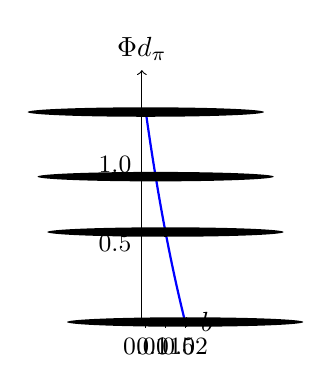
\begin{tikzpicture}[x=50cm,y=2cm]
\draw[->] (0.009,0) -- (0.0215,0) node[right] {$b$};
\draw[->] (0.009,0) -- (0.009,1.6) node[above] {$\Phi d_\pi$};
\foreach \b in {0.01,0.015,0.02} \draw (\b,0) -- (\b,-0.04) node[below] {\small\b};
\foreach \v in {0.5,1.0} \draw (0.009,\v) -- (0.0088,\v) node[left] {\small\v};
\draw[thick,blue] plot[domain=0.01:0.02,samples=40] (\x,{4*(0.02-\x)/(\x+0.02)});
\foreach \b/\v in {0.01/1.3333,0.0125/0.9231,0.015/0.5714,0.02/0} \fill (\b,\v) circle (0.03);
\end{tikzpicture}
\end{center}
The curve is decreasing and convex. Rebalancing the \emph{direction} of dependence ($b \to 0.02$) removes the recurring transfer altogether: at $b = 0.02$ the matrix is doubly stochastic.

\solpart{c} Multiplying all cross-block entries by 5 gives $\varepsilon_1 = 10b$ and $\varepsilon_2 = 0.2$. The block mass $\varepsilon_2/(\varepsilon_1+\varepsilon_2) = 0.2/(10b + 0.2)$ is unchanged, so $\boldsymbol\pi$, $\x^*$, $\Phi d_\pi$ and $L_{\text{power}}$ are the same as in~(b), for every $b$. What changes is the spectral gap. The lumped $2\times2$ chain has second eigenvalue $1 - \varepsilon_1 - \varepsilon_2$, and the within-block deviation vectors ($x_1 = -x_2$ or $x_3 = -x_4$) have eigenvalue 0, because within-block weights are equal. So the spectrum is $\{1, 1 - \varepsilon_1 - \varepsilon_2, 0, 0\}$ and $\Gamma = \varepsilon_1 + \varepsilon_2$:
\begin{center}
\begin{tabular}{ccccc}
\toprule
$b$ & 0.0100 & 0.0125 & 0.0150 & 0.0200 \\
\midrule
$\Gamma$ (original) & 0.060 & 0.065 & 0.070 & 0.080 \\
$\Gamma$ (cross entries $\times5$) & 0.300 & 0.325 & 0.350 & 0.400 \\
\bottomrule
\end{tabular}
\end{center}
\emph{Why:} power depends on the \emph{ratio} of the cross-block flows, integration on their \emph{level} (Chapter~3, Proposition~\ref{ch03:prop:block_spectral}). Scaling every cross flow by the same factor is ``integration only'' (Policy~B1 of the example): it speeds up mixing and does nothing for the distribution.

%% ---------------------------------------------------------------------
\exercisesolution{2.3}{Welfare decomposition}

Parameters: $m = \Omega/N = 1$, $1 - \kappa m = 0.5$, $\gamma = 0.5$, $\Phi = 1$. We use Theorem~\ref{ch02:thm:welfare_loss} with $c_j = \sum_{i\neq j}W_{ij}$ (off-diagonal column sums; the diagonal never enters~\eqref{ch02:eq:social_utility}), $\alpha_j = 1 + \gamma c_j$, $H = N/\sum_j\alpha_j^{-1}$, and the exact formula~\eqref{ch02:eq:ext_loss}.

\solpart{a} For $W = \frac13\ones\ones'$: $\boldsymbol\pi = \frac13\ones$, so $\Var(\pi_i) = 0$ and $L_{\text{power}} = 0$. Every $c_j = \frac23$, so all $\alpha_j = \frac43 = H$ and $L_{\text{externality}} = \frac{(1-\kappa m)^2}{2\kappa}\sum_j(\alpha_j - H)^2/\alpha_j = 0$. Both terms of $L_{\text{interaction}}$ contain $\pi_j - \frac13$ or $\Cov(\pi_j, c_j)$, so it vanishes too. The social optimum and the bargaining allocation are both $(1,1,1)$.

\solpart{b} The Perron vector is $\boldsymbol\pi = (0.2340, 0.4043, 0.3617)$, with $\Var(\pi_i) = 0.005231$ and $\Neff = 2.8651$. (The full column sums are $(0.8, 1.2, 1.0)$, so $W$ is not doubly stochastic.) The off-diagonal column sums are
\begin{gather*}
\mathbf c = (0.2 + 0.1,\ 0.4 + 0.3,\ 0.1 + 0.3) = (0.3, 0.7, 0.4),\\
\Var(c_j) = 0.028889,\qquad \Cov(\pi_j, c_j) = 0.010402,
\end{gather*}
so $\boldsymbol\alpha = (1.15, 1.35, 1.20)$ and $H = 1.227677$. The three terms:
\begin{align*}
L_{\text{externality}} &= \tfrac{0.25}{1}\textstyle\sum_j (\alpha_j - H)^2/\alpha_j = 0.004242,\\
L_{\text{power}} &= \tfrac{\kappa N}{2}\Phi^2\Var(\pi_i) = 0.75 \times 0.005231 = 0.003923,\\
L_{\text{interaction}} &= \underbrace{\tfrac{\kappa\gamma\Phi^2}{2}\textstyle\sum_j c_j(\pi_j - \tfrac13)^2}_{0.000850}\ \underbrace{-\,\gamma\Phi N(1 - \kappa m)\Cov(\pi_j, c_j)}_{-0.007801}\\
&= -0.006951 .
\end{align*}
The second-order approximation to $L_{\text{externality}}$ in~\eqref{ch02:eq:ext_loss} gives $0.005417$; $\gamma = 0.5$ is not small.
The total is $L = 0.001214$. The script confirms it directly as $\sum_j\alpha_jU(x^{\text{soc}}_j) - \sum_j\alpha_jU(x^{\text{barg}}_j)$, with social optimum $\x^{\text{soc}} = (0.9325, 1.0906, 0.9769)$ (Proposition~\ref{ch02:prop:ext_loss}) and bargaining allocation $\x^{\text{barg}} = (0.9007, 1.0709, 1.0284)$. Both satisfy $\kappa x_j \le 0.545 < 1$, so the interior hypothesis of the theorem holds.

\solpart{c} $L_{\text{interaction}} = -0.006951 < 0$. It is negative because $\Cov(\pi_j, c_j) > 0$: agent~2 is both the most powerful ($\pi_2 = 0.4043$) and the most cared about ($c_2 = 0.7$). The bargaining tilt toward her is in the same direction as the planner's tilt toward the agent whose consumption others value, so the two distortions partly cancel. The tilt even overshoots the social optimum for agent~3 ($1.0284 > 0.9769$), which is why $L_{\text{interaction}}$ cannot cancel everything. If power sat with agents nobody cares about ($\Cov < 0$), the interaction term would be positive and the losses would compound. \emph{Common mistake:} reading $L_{\text{interaction}} < 0$ as ``power is good''. It says only that, \emph{under a social welfare function that counts the caring}, part of the power tilt is endorsed; whether such caring should count is normative (Chapter~2, Section~\ref{ch02:sec:decomposition}).

%% ---------------------------------------------------------------------
\exercisesolution{2.4}{Spectral gap across topologies}

The constructions, for $N = 8$:
\begin{itemize}
\item (a) $W^{CE} = \frac18\ones\ones'$.
\item (b) The undirected ring: $W_{i,i\pm1} = \frac12$ (indices mod 8), no self-loops.
\item (c) Two blocks: $W = \text{diag}(\frac14\ones_4\ones_4', \frac14\ones_4\ones_4')$.
\item (d) The star: the spokes put weight 1 on the hub, and the hub spreads $\frac17$ over the spokes ($a = 1$, $s = 0$ in Chapter~6, Proposition~\ref{ch06:prop:star_power}).
\end{itemize}
\begin{center}
\begin{tabular}{lcccccc}
\toprule
& \multicolumn{3}{c}{$W$} & \multicolumn{3}{c}{lazy $\frac12(I + W)$}\\
\cmidrule(lr){2-4}\cmidrule(lr){5-7}
& $\Gamma$ & $\Neff$ & $\Var(\pi)$ & $\Gamma$ & $\Neff$ & $\Var(\pi)$ \\
\midrule
(a) $W^{CE}$ & 1 & 8 & 0 & 0.5 & 8 & 0\\
(b) ring & 0 & 8 & 0 & 0.1464 & 8 & 0 \\
(c) two blocks & 0 & --- & --- & 0 & --- & --- \\
(d) star & 0 & 3.5 & 0.02009 & 0.5 & 3.5 & 0.02009 \\
\bottomrule
\end{tabular}
\end{center}

\emph{Details.}
\begin{itemize}
\item (b) The ring is a circulant with eigenvalues $\cos(2\pi k/8)$, $k = 0, \ldots, 7$: $1, 0.7071, 0, -0.7071, -1, \ldots$. It is doubly stochastic, so $\boldsymbol\pi$ is uniform.
\item (d) Power concentrates on the hub: $\pi_h = a/(a + 1 - s) = \frac12$, each spoke has $\frac{1}{14} = 0.0714$, and $\Neff = 1/(\frac14 + 7\cdot\frac{1}{196}) = 3.5$.
\item Lazy versions: the eigenvalues map as $\lambda \mapsto (1+\lambda)/2$, so the lazy ring has $\lambda_2 = (1 + \cos\frac\pi4)/2 = 0.8536$, and the lazy star has spectrum $\{1, 0.5^{(6)}, 0\}$, matching Proposition~\ref{ch06:prop:star_power} with $a = s = \frac12$. Laziness never changes $\boldsymbol\pi$, since $\boldsymbol\pi'\frac12(I+W) = \boldsymbol\pi'$.
\end{itemize}

\emph{Why the ring and the star have $\Gamma = 0$ although they are connected.} Both are irreducible but \emph{periodic}: their graphs are bipartite. For the ring, colour the nodes alternately $\pm1$; $\x = (1,-1,1,-1,\ldots)'$ satisfies $(W\x)_i = \frac12(x_{i-1} + x_{i+1}) = -x_i$. For the star, $\x$ with $x_h = 1$ and $x_{\text{spoke}} = -1$ gives $(W\x)_h = 7\cdot\frac17(-1) = -x_h$ and $(W\x)_{\text{spoke}} = x_h = -x_{\text{spoke}}$. In both cases $-1$ is an eigenvalue, $|\lambda_2| = 1$, and $\Gamma = 0$: deviations oscillate forever instead of decaying (Chapter~6, Theorem~\ref{ch06:thm:PF}, item~5). The directed ring $i \to i+1$ is periodic with period 8 and also has $\Gamma = 0$. A self-loop breaks the periodicity, which is what laziness does.

\emph{Why the two blocks have no unique $\boldsymbol\pi$.} The matrix is reducible, and each block is a closed class with its own stationary vector $\frac14\ones_4$. Hence $(\frac14\ones_4', 0)$, $(0, \frac14\ones_4')$ and every convex combination $(t\cdot\frac14\ones_4', (1-t)\cdot\frac14\ones_4')$ are stationary; the eigenvalue 1 has multiplicity 2 (Chapter~3, Proposition~\ref{ch03:prop:block_spectral}(1)). $\Neff$ ranges from 4 to 8 depending on $t$, so ``power'' is undefined until the blocks are coupled.

\emph{Do $\Gamma$ and $\Neff$ move together?} No. The lazy $W^{CE}$ and the lazy star have the same $\Gamma = 0.5$ with $\Neff = 8$ and $3.5$. The ring and $W^{CE}$ have the same $\Neff = 8$ with $\Gamma = 0$ and $1$. Making a matrix lazy halves its distance from 1 in the spectrum (it lowers $\Gamma$ of $W^{CE}$ from 1 to 0.5 and raises that of the star from 0 to 0.5) without touching $\boldsymbol\pi$. This is Chapter~6, Proposition~\ref{ch06:prop:gap-power-independent} in action.

%% ---------------------------------------------------------------------
\exercisesolution{2.5}{Block disconnection with data}

\textbf{Data (real results, with a stated limitation).}
\begin{itemize}
\item \textbf{Value added.} Gross value added by sector, 2019, from INE's supply-use tables, base 2017, aggregated to the book's 12 sectors \citep{ine2026sut} (\texttt{data/processed/bolivia\_io\_sector\_facts.csv}, million current Bs).
\item \textbf{Employment.} Employment by ISIC Rev.~4 section, 2019, from ILOSTAT \citep{ilo2026ilostat}, which processes INE's Encuesta Continua de Empleo microdata (\texttt{data/processed/ilostat\_bolivia\_emp\_eco\_sex.csv}, thousands of persons).
\end{itemize}
Both were retrieved 2026-11-05.

\textbf{Method.}
\begin{enumerate}
\item \emph{Map sectors to ISIC sections.} Hydrocarbons and Mining together form section~B. The other matches are: Agriculture A, Manufacturing C, Construction F, Commerce G, Transport H, Financial services K, Personal services I+R+S, Domestic services T. INE puts non-market education and health in Public administration, so Public administration and Other services are merged and matched to D+E+J+L+M+N+O+P+Q+U. The mapped employment adds to the ILOSTAT total of 5{,}622.1 thousand.
\item \emph{Value added per worker} $y_g = \text{VA}_g/n_g$, in Bs per worker per year.
\item \emph{Two blocks:} B (Hydrocarbons + Mining) and everything else. Compute the employment-weighted between-group variance $\sum_b \frac{n_b}{n}(\bar y_b - \bar y)^2$ and the within-group component of Appendix~\ref{ch02:app:variance}, using the nine sector means inside block~2.
\end{enumerate}

\textbf{Results.}
\begin{center}
\small
\begin{tabular}{lrrr}
\toprule
& VA (million Bs) & workers (thousand) & VA per worker (Bs)\\
\midrule
Hydrocarbons + Mining & 34{,}923.3 & 75.2 & 464{,}610 \\
Everything else & & 5{,}546.9 & 49{,}585 \\
Economy & & 5{,}622.1 & 55{,}134 \\
\bottomrule
\end{tabular}
\end{center}
Value added per worker in the extractive block is $9.37$ times that of the rest, and the block employs $1.34\%$ of workers. Variance of VA per worker (Bs$^2$):
\begin{itemize}
\item between blocks: $2.2721\times10^{9}$;
\item within block~2, across sectors: $1.9458\times10^{9}$ (driven by financial services, $378{,}118$ Bs per worker, and public administration plus other services, $122{,}495$);
\item total: $4.2180\times10^{9}$.
\end{itemize}
The between-group share is $0.5387$ and the ratio between/within is $1.1677$. By Proposition~\ref{ch02:prop:block_loss}, $L_{\text{block}} = \frac{\kappa}{2}n\cdot(\text{between variance})$, so the ratio of $L_{\text{block}}$ to the within-group loss is the same $1.1677$ for every $\kappa$. For a scale: with $\kappa = 10^{-6}$ per Bs ($\kappa y_g \le 0.465 < 1$ for every sector), $L_{\text{block}}$ is $1{,}136$ utility units per worker, against $973$ within.

\textbf{Interpretation.}
\begin{itemize}
\item \emph{Levels versus logs.} The between-block term is large in levels because a tiny, extremely capital-intensive block sits far above the mean. In logs, which weight proportional gaps, the between share falls to $0.1477$ (between $0.0828$, within $0.4776$). The ``two-block'' diagnosis is sensitive to the metric.
\item \emph{VA is not income.} Compensation of employees is only $5.95\%$ of hydrocarbons' value added ($29.13\%$ in mining), and compensation per worker in the block is $76{,}662$ Bs a year. Most of the block's VA per worker is rent and capital income, which reaches households through the state (Chapter~3), not through the workers.
\item \emph{Lower bound.} The within component here is across sectors only. True within-group dispersion across individuals is larger and needs household-survey microdata (INE's Encuesta de Hogares), which were not fetched. The between share reported is therefore an upper bound on the share in an individual-level decomposition.
\end{itemize}

%% ---------------------------------------------------------------------
\exercisesolution{2.6}{El Alto vs.\ Zona Sur}

\illustrative\ The figures are the exercise's, not survey estimates.

\solpart{a} $\bar\omega = (5\cdot800 + 3\cdot4500)/8 = 2187.5$ Bs. By Proposition~\ref{ch02:prop:block_loss},
\[
\begin{aligned}
L_{\text{block}} &= \frac{0.0001}{2}\bigl[5(800 - 2187.5)^2 + 3(4500 - 2187.5)^2\bigr]\\
&= 0.00005\,(9{,}625{,}781.25 + 16{,}042{,}968.75) = 1283.4375 .
\end{aligned}
\]
Satiation check: $\kappa\bar\omega_{\text{Alto}} = 0.08$ and $\kappa\bar\omega_{\text{Sur}} = 0.45$, both $< 1$.

\solpart{b} Each El Alto agent puts total weight $\varepsilon_1 = 3\varepsilon$ on Zona Sur and $(1 - 3\varepsilon)/5$ on each El Alto agent. Each Zona Sur agent puts $\varepsilon_2 = 5\varepsilon$ on El Alto and $(1 - 5\varepsilon)/3$ on each Zona Sur agent. The partition is exactly lumpable, so $1 - \varepsilon_1 - \varepsilon_2 = 1 - 8\varepsilon$ is an eigenvalue (Proposition~\ref{ch06:prop:block_power}). Any vector supported on one block and summing to zero there is mapped to zero, because within-block weights are equal. The spectrum is therefore $\{1, 1 - 8\varepsilon, 0^{(6)}\}$ and $\Gamma = 1 - |1 - 8\varepsilon|$:
\begin{itemize}
\item $\varepsilon = 0.02$: $\lambda_2 = 0.84$, $\Gamma = 0.16$; cross-block deviations halve in $3.976$ periods.
\item $\varepsilon = 0.15$: $\lambda_2 = -0.2$, $\Gamma = 0.80$; they halve in $0.431$ periods, and the sign alternates.
\end{itemize}
$L_{\text{block}}$ is $1283.4375$ in both cases. $\Gamma$ is a property of how fast an averaging process on $W$ (beliefs, prices, norms) mixes across the blocks. $L_{\text{block}}$ is a property of where \emph{resources} are: it compares within-block equal division with full equal division and contains no $W$ at all. A faster-mixing information network does not move a single boliviano from Zona Sur to El Alto. Integration lowers $L_{\text{block}}$ only through a mechanism that makes resources cross: labour mobility, cross-block trade at better terms, fiscal transfers.

Two more facts. Column sums are $5\cdot\frac{1 - 3\varepsilon}{5} + 3\varepsilon = 1$ for El Alto and $5\varepsilon + 3\cdot\frac{1-5\varepsilon}{3} = 1$ for Zona Sur, so $W$ is doubly stochastic and $\boldsymbol\pi = \frac18\ones$ ($\Neff = 8$) for every $\varepsilon$. Equivalently, the block mass $\varepsilon_2/(\varepsilon_1 + \varepsilon_2) = 5/8$ equals El Alto's population share. This economy has segregation and slow integration without any power concentration.

\solpart{c} $\varepsilon$ is the weight each agent puts on the other block: in information terms, how much people in El Alto hear, see and rely on people in Zona Sur, and vice versa. Interventions that raise it create repeated cross-block contact:
\begin{itemize}
\item urban transport that cuts travel time between the blocks, such as the Mi Telef\'erico cable-car network linking El Alto and La Paz (opened 2014);
\item socially mixed schools and universities;
\item hiring and procurement that cross the blocks (public employment, supplier programmes);
\item shared media and public spaces.
\end{itemize}
A strong answer distinguishes interventions that raise $\varepsilon$ (contact, integration) from those that close the gap in block means (transfers, labour-market integration). Only the second lower $L_{\text{block}}$ directly, though the first may help the second happen.

%% ---------------------------------------------------------------------
\exercisesolution{2.7}{Furtado's thesis formalized}

\solpart{a} \textbf{A two-block economy with self-reproducing disconnection.} Aggregate the economy into two blocks, Modern ($M$) and Traditional ($T$), with
\[
W_t = \begin{pmatrix} 1 - \varepsilon_t & \varepsilon_t \\ \varepsilon_t & 1 - \varepsilon_t\end{pmatrix}, \qquad \x^*(W_t) = W_t\boldsymbol\omega ,
\]
so the traditional block's income is $x_T(\varepsilon) = \omega_T + \varepsilon(\omega_M - \omega_T)$: coupling lets part of the modern block's resources reach the traditional one. Linkages are built out of the traditional block's surplus over subsistence $\bar c$, with a cap $I_{\max}$ on what one period's surplus can finance, and depreciate at rate $\delta$ toward a floor $\varepsilon_0$ (minimal trade):
\[
\varepsilon_{t+1} = f(\varepsilon_t) = (1-\delta)\varepsilon_t + \delta\varepsilon_0 + \sigma\min\{\max\{x_T(\varepsilon_t) - \bar c, 0\},\ I_{\max}\}.
\]
This is $W_{t+1} = f(W_t, \x^*(W_t))$. \illustrative\ Parameters: $\omega_M = 8$ and $\omega_T = 3.2$ (Example~\ref{ch02:ex:two_blocks}), $\bar c = 3.5$, $\delta = 0.1$, $\sigma = 0.05$, $\varepsilon_0 = 0.02$, $I_{\max} = 0.5$.

\emph{The block-diagonal fixed point.} The traditional block starts investing only above $\varepsilon_{\text{th}} = (\bar c - \omega_T)/(\omega_M - \omega_T) = 0.0625$. Below it, $f(\varepsilon) = (1 - \delta)\varepsilon + \delta\varepsilon_0$, whose fixed point is $\varepsilon^* = \varepsilon_0 = 0.02$. There, traditional income is $3.2960 < \bar c = 3.5$: the structure produces an allocation too poor to finance the linkages that would change the structure. This $W^*$ has weak coupling and, with the block means of Example~\ref{ch02:ex:two_blocks}, $L_{\text{block}} = 2.16 > 0$ (Proposition~\ref{ch02:prop:block_loss}).

The map has two more fixed points. Between the threshold and saturation ($\varepsilon \le 0.1667$), $\delta(\varepsilon - \varepsilon_0) = \sigma(x_T(\varepsilon) - \bar c)$ gives the middle one,
\[
\hat\varepsilon = \frac{\sigma(\bar c - \omega_T) - \delta\varepsilon_0}{\sigma(\omega_M - \omega_T) - \delta} = 0.0929 .
\]
Above saturation, $\varepsilon_{\text{high}} = \varepsilon_0 + \sigma I_{\max}/\delta = 0.27$. The script verifies $f(\varepsilon) = \varepsilon$ at all three.

\solpart{b} \textbf{Stability.} $f$ is piecewise linear with slope $1 - \delta = 0.9$ below the threshold and above saturation, and slope $1 - \delta + \sigma(\omega_M - \omega_T) = 1.14$ in between. A fixed point of a one-dimensional map is locally stable when $|f'(\varepsilon^*)| < 1$. So:
\begin{itemize}
\item $\varepsilon^* = 0.02$ is stable, with basin $[0, 0.0929)$;
\item $\hat\varepsilon = 0.0929$ is unstable (the threshold between the two basins);
\item $\varepsilon_{\text{high}} = 0.27$ is stable, with basin $(0.0929, 1]$.
\end{itemize}
Simulations: starting at $0.05$ or $0.09$ the coupling returns to $0.02$; starting at $0.095$ or $0.15$ it converges to $0.27$. In general, the underdevelopment fixed point $W^*$ is stable when two conditions hold:
\begin{enumerate}
\item At $W^*$ the allocation leaves the traditional block below its investment threshold: $\varepsilon_0(\omega_M - \omega_T) < \bar c - \omega_T$.
\item Small increases in coupling do not raise investment faster than linkages depreciate: $|1 - \delta + \sigma\,\partial x_T/\partial\varepsilon| < 1$ at $W^*$. Here $\partial(\text{investment})/\partial\varepsilon = 0$ below the threshold, so this reduces to $\delta > 0$.
\end{enumerate}
For a matrix-valued map, the condition is that the Jacobian of $W \mapsto f(W, \x^*(W))$, restricted to perturbations $E$ with $E\ones = 0$ (which keep rows stochastic), has spectral radius below one at $W^*$. The case study's smooth map $F(\varepsilon) = \bar\varepsilon\varepsilon^2/(\varepsilon^2 + h^2)$ has the same three-fixed-point structure.

\solpart{c} \textbf{Breaking out} means leaving the basin of $W^*$. There are two ways.
\begin{enumerate}
\item \emph{A big push in the state.} Raise $\varepsilon$ past the unstable threshold, a one-off jump of at least $\hat\varepsilon - \varepsilon_0 = 0.0729$ in coupling. A one-off income transfer cannot do this here. It raises next period's coupling by at most $\sigma I_{\max} = 0.025$, and the script confirms that one-off transfers of $0.5$ to $2$ all return to $\varepsilon = 0.02$. This is the dynamic counterpart of Proposition~\ref{ch02:thm:transfer_trap}: transfers move $\x$, not $W$.
\item \emph{A change in parameters that destroys the low fixed point} (a bifurcation). A permanent rise of $0.2040$ in $\omega_T$, a lower subsistence threshold, or a higher floor $\varepsilon_0$ (a public linkage programme) all make condition~1 fail, so that only the high equilibrium remains.
\end{enumerate}
In Furtado's terms, underdevelopment is not a stage but a basin of attraction, and development is a structural change large enough to cross its boundary. \emph{Common mistake:} identifying ``breaking out'' with growth of $\omega_M$. Modern-sector growth reaches the traditional block only through the floor coupling: it raises $x_T(\varepsilon_0) = \omega_T + \varepsilon_0(\omega_M - \omega_T)$, and here it removes the trap only if $\omega_M > 18.20$, more than doubling the modern endowment. With $\varepsilon_0 = 0$, no growth of $\omega_M$ helps at all.

\end{document}
